\section{About Libraries}

% Details on implementation. 
% Architecture.

% TODO:
% - stunning architecture diagram
% - exciting example of usage
% - unbelievable python API showcase 

Implemented sparse boolean linear algebra libraries for OpenCL and NVIDIA Cuda platforms are called
\textit{clBool}\footnote{clBool project: \url{https://replace/me/with/actual/url}. Access date: 03.02.2021.} and \textit{cuBool}\footnote{cuBool project: \url{https://github.com/JetBrains-Research/cuBool}. Access date: 03.02.2021.} respectively.
Projects are hosted at GitHub platform. The source code is licensed under MIT license.
The build process is straightforward: it is configured with CMake tool and requires extra setup only of platform-specific development kits. 

Libraries architecture is briefly depicted at figure~\ref{fig:generic_architecture}. 
The core of the libraries is written in the C++ programming languages, which is well-suited for performance and resource critical computational tasks. 
Actual GPU related logic is presented in platform specific backends: Cuda and OpenCL, which use respective technologies for resources and GPU executable code management.
cuBool library exposes C compatible API, what gives expressiveness and allows to embed that API into other execution environments by interoperability mechanisms. 
Pycubool module encapsulates such functionality and provides it for high-level Python runtime.

It is worth mention, that it is convenient to create the single library with common interface and several backends for different execution targets.
At this time clBool and cuBool are distinct libraries, but they can be integrated into single library.
This integration is something to be done in near future.
This process requires careful selection of the interface to allow the end user properly configure the library for specific tasks, as well as provide the option to automatically select a specific implementation depending on the capabilities of the target device.

\begin{figure}[t]
    \centering
    % Todo: maybe draw this diagram more compact (vertically)
    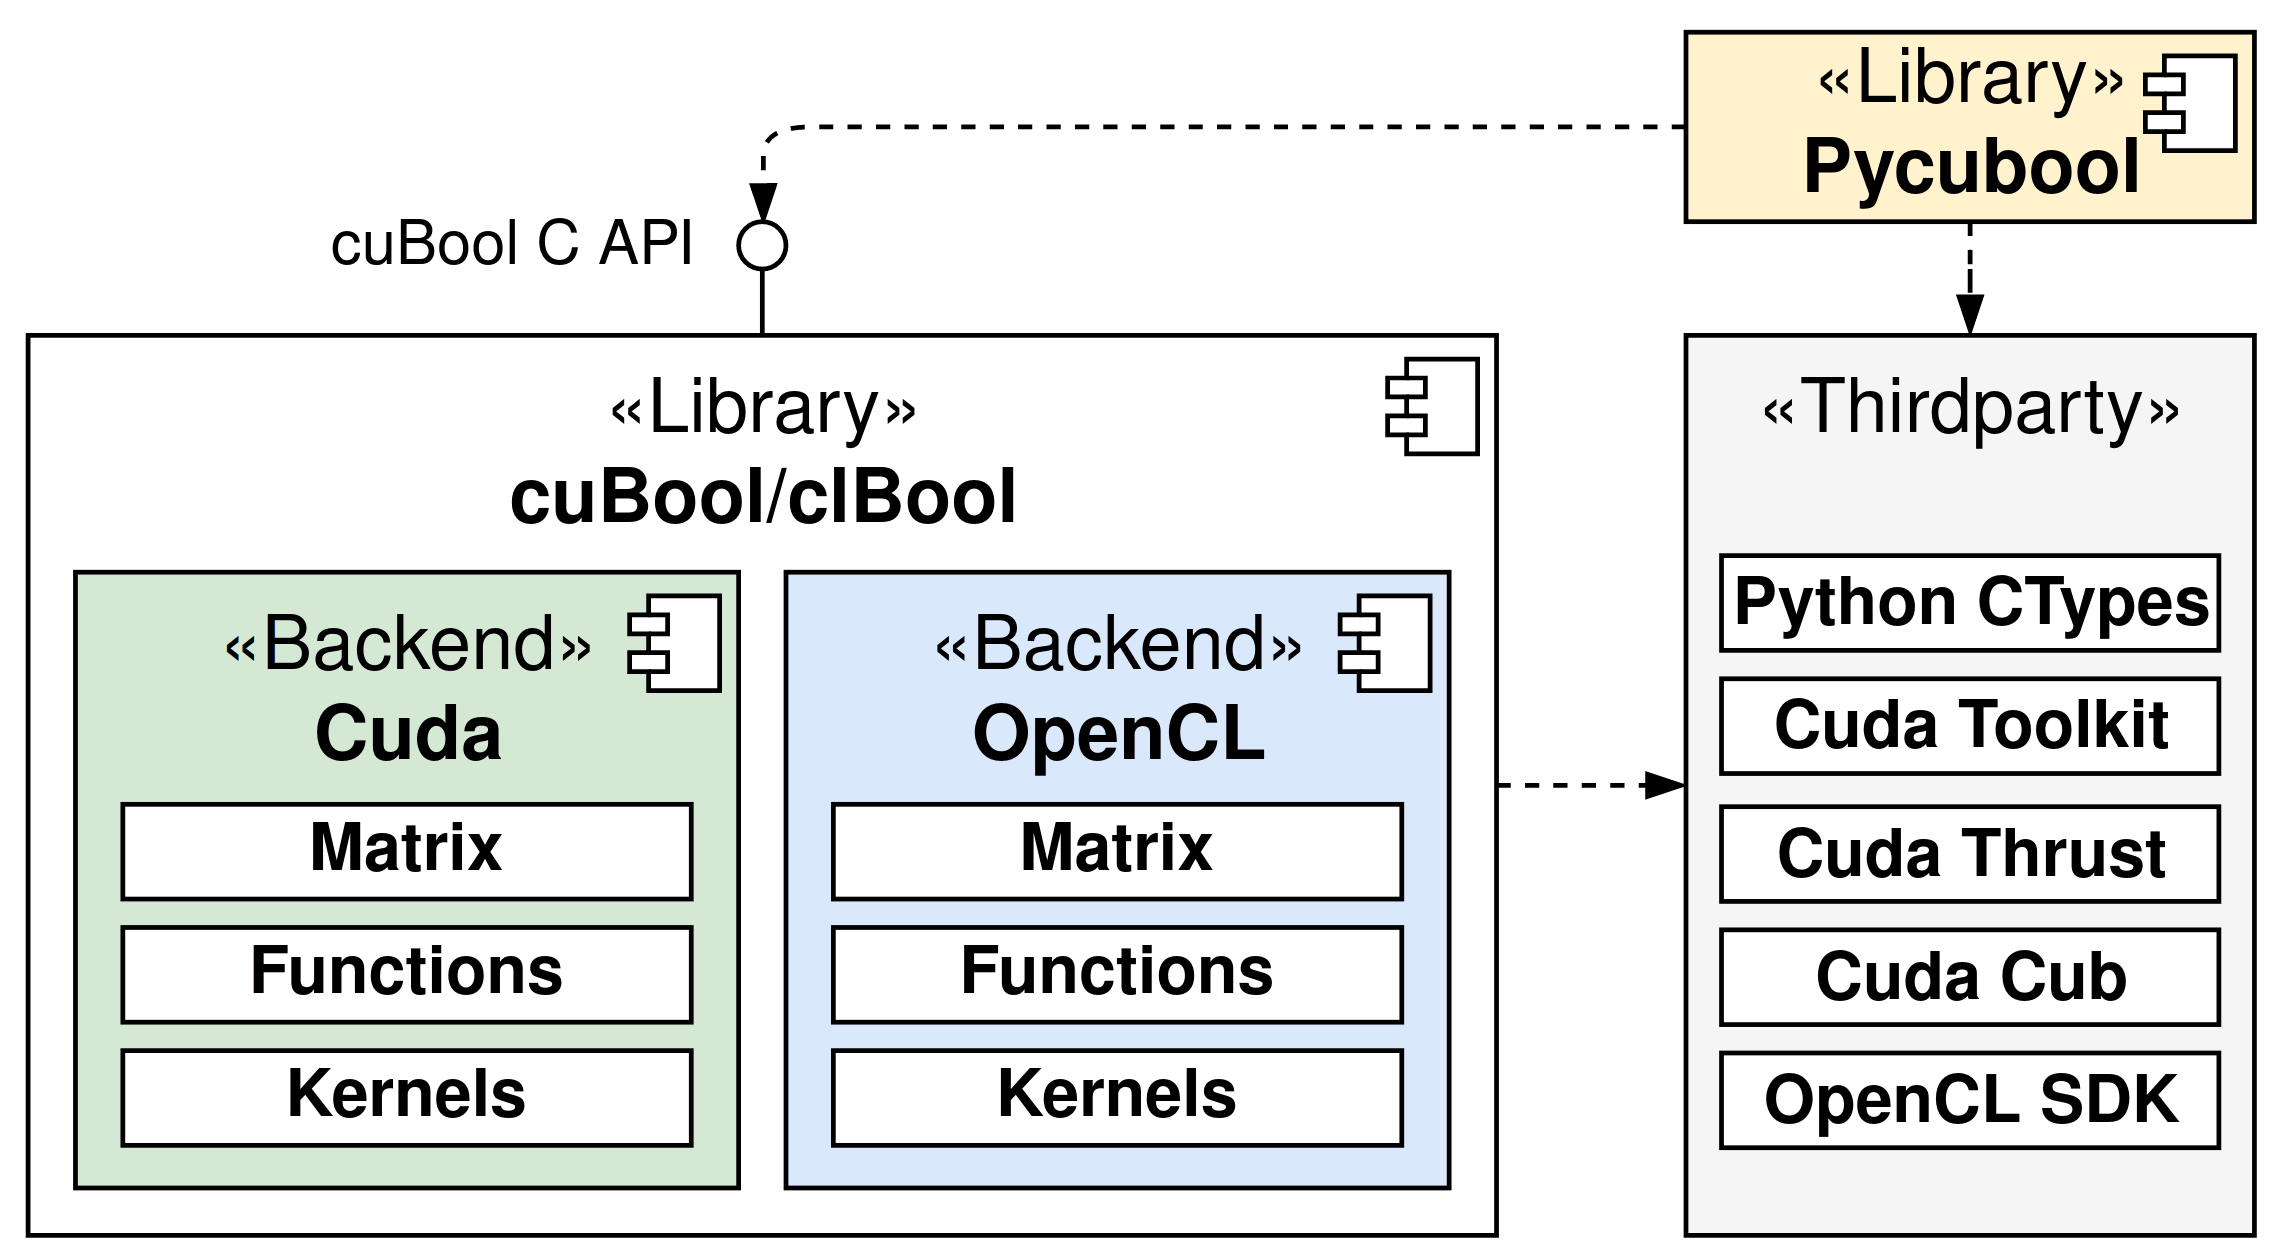
\includegraphics[width=0.4\textwidth]{generic_architecture.png}
    \caption{Conceptual sparse boolean linear algebra library architecture}
    \label{fig:generic_architecture}
\end{figure}

Libraries operate on boolean semiring with values set \{\textit{true}, \textit{false}\} with \textit{false} as 
a neutral element, '+' operation defined as logical \textit{or} and '*' defined as logical \textit{and}. Values are also denoted as $\{1,~0\}$ respectively, and the abbreviation $\textit{nnz(M)}$ gives the number of non-zero cells of the matrix $M$.

Main primitive is sparse matrix of boolean values, stored in one of the sparse formats. Sparse vector 
primitive is not presented, since its utilization is relatively rare presented in practical computational 
tasks. But its support is something to be added in far future. Primary available operations and functions are following.

\begin{itemize}
    \item Create sparse matrix $M$ of size $m \times n$.
    \item Delete sparse matrix $M$ and release all its internal resources.
    \item Fill the matrix $M$ with values $L = \{(i,j)_k\}_k$. The result of this operation is $M_{i,j} = 1$ for each $(i, j) \in L$, and $M_{i,j} = 0$ for the rest of matrix values.
    \item Read matrix $M$ values $L = \{(i, j)~|~M_{i,j} = 1\}$.
    \item Matrix-matrix multiply-add operation $C \mathrel{+}= M \times N$.
    \item Matrix-matrix add operation $M \mathrel{+}= N$.
    \item Matrix-matrix Kronecker product $K = M \otimes N$.
\end{itemize}